\documentclass[11pt,a4paper]{article}
\usepackage[spanish,es-nodecimaldot]{babel}	% Utilizar español
\usepackage[utf8]{inputenc}					% Caracteres UTF-8
\usepackage{graphicx}						% Imagenes
\usepackage[hidelinks]{hyperref}			% Poner enlaces sin marcarlos en rojo
\usepackage{fancyhdr}						% Modificar encabezados y pies de pagina
\usepackage{float}							% Insertar figuras
\usepackage[textwidth=390pt]{geometry}		% Anchura de la pagina
\usepackage[nottoc]{tocbibind}				% Referencias (no incluir num pagina indice en Indice)
\usepackage{enumitem}						% Permitir enumerate con distintos simbolos
\usepackage[T1]{fontenc}					% Usar textsc en sections
\usepackage{amsmath}						% Símbolos matemáticos
\usepackage{listings}
\usepackage{color}

 
\definecolor{codegreen}{rgb}{0,0.6,0}
\definecolor{codegray}{rgb}{0.5,0.5,0.5}
\definecolor{codepurple}{rgb}{0.58,0,0.82}
\definecolor{backcolour}{rgb}{0.99,0.99,0.99}
 
\lstdefinestyle{mystyle}{
    backgroundcolor=\color{backcolour},   
    commentstyle=\color{codegreen},
    keywordstyle=\color{magenta},
    numberstyle=\tiny\color{codegray},
    stringstyle=\color{codepurple},
    basicstyle=\footnotesize,
    breakatwhitespace=false,         
    breaklines=true,                 
    captionpos=b,                    
    keepspaces=true,                 
    numbers=left,                    
    numbersep=5pt,                  
    showspaces=false,                
    showstringspaces=false,
    showtabs=false,                  
    tabsize=2
}
 
\lstset{style=mystyle, language=Python}

% Comando para poner el nombre de la asignatura
\newcommand{\asignatura}{Inteligencia de Negocio}
\newcommand{\autor}{José María Sánchez Guerrero}
\newcommand{\titulo}{Práctica 3}
\newcommand{\subtitulo}{Competición en Kaggle}

% Configuracion de encabezados y pies de pagina
\pagestyle{fancy}
\lhead{\autor{}}
\rhead{\asignatura{}}
\lfoot{Grado en Ingeniería Informática}
\cfoot{}
\rfoot{\thepage}
\renewcommand{\headrulewidth}{0.4pt}		% Linea cabeza de pagina
\renewcommand{\footrulewidth}{0.4pt}		% Linea pie de pagina

\begin{document}
\pagenumbering{gobble}

% Pagina de titulo
\begin{titlepage}

\begin{minipage}{\textwidth}

\centering


\includegraphics[scale=0.5]{img/ugr.png}\\

\textsc{\Large \asignatura{}\\[0.2cm]}
\textsc{GRADO EN INGENIERÍA INFORMÁTICA}\\[1cm]

\noindent\rule[-1ex]{\textwidth}{1pt}\\[1.5ex]
\textsc{{\Huge \titulo\\[0.5ex]}}
\textsc{{\Large \subtitulo\\}}
\noindent\rule[-1ex]{\textwidth}{2pt}\\[3.5ex]

\end{minipage}

\vspace{0.5cm}

\begin{minipage}{\textwidth}

\centering

\textbf{Autor}\\ {\autor{}}\\[2.5ex]
\textbf{Rama}\\ {Sistemas de Información}\\[2.5ex]
\vspace{0.3cm}


\includegraphics[scale=0.3]{img/etsiit.jpeg}

\vspace{0.3cm}
\textsc{Escuela Técnica Superior de Ingenierías Informática y de Telecomunicación}\\
\vspace{1cm}
\textsc{Curso 2020-2021}
\end{minipage}
\end{titlepage}

\begin{figure}[H]
    \centering
    \hspace*{-0.5in}
    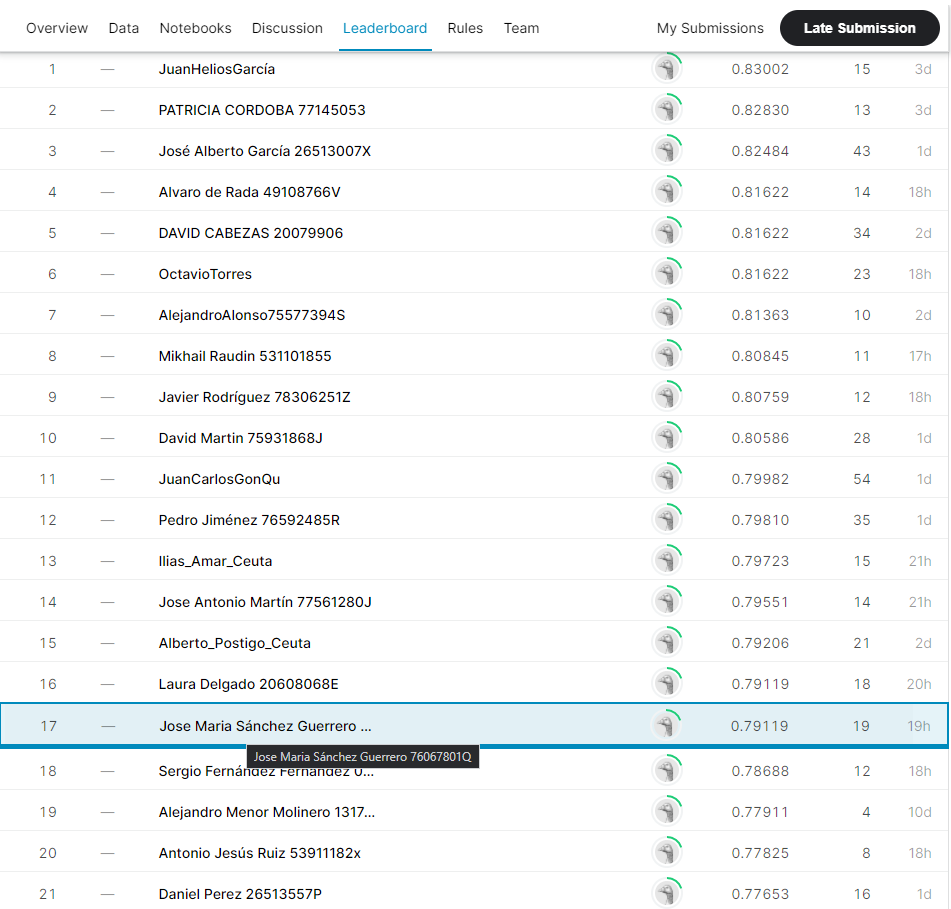
\includegraphics[scale=0.65]{img/leaderboard.png}
\end{figure}

\newpage

\pagenumbering{arabic}
\tableofcontents
\thispagestyle{empty}				% No usar estilo en la pagina de indice

\newpage

\setlength{\parskip}{1em}



\section{Introducción}

En esta última práctica pondremos a prueba lo aprendido en las prácticas anteriores a través de una competición en la plataforma
Kaggle. En ella se nos plantea un problema de clasificación de una serie de coches vendidos, donde tendremos que predecir la
categoría del precio del coche (del 1 al 5, yendo de más barato a más caro), por lo tanto estamos ante un problema de clasificación
multiclase.

Dispondremos de un conjunto de entrenamiento, con 4819 ejemplos de coches vendidos y el precio con el que fueron vendidos; y un
conjunto de test, con 1158 ejemplos de coches vendidos y los cuales tendremos que predecir el precio al que se vendieron. Este
resultado será el que subiremos a la web para comprobar que tal ha funcionado la estrategia que hemos seguido. Para medir el
rendimiento se utilizará la precisión ($accuracy$) obtenida.


\section{Estrategias y progreso obtenido}

Como no se ha seguido una estrategia planeada, si no que se ha ido modificando dependiendo de los resultados obtenidos, vamos a
explicar poco a poco que métodos hemos utilizado y cómo los hemos mejorado. En algunos casos no se ha podido mejorar, no obstante,
también explicaremos que se había intentado y por qué.

\subsection{Primeros pasos}

En primer lugar, intentamos comprender los datos, ver con qué estamos trabajando y explorar los distintos métodos que tenemos a
nuestra disposición para resolverlo. Se utiliza un sólo $script$ para esta parte ('\textit{primeros-pasos.ipynb}'), ya que entre
unas ejecuciones y otras se cambiaban unos parámetros, o bien, se ejecutan a la vez.

\phantomsection
\label{pp1}
Para empezar, nada más leer el dataset, vemos que hay bastantes datos que faltan o datos nulos. Unos 72 o más por atributo, y
hasta 4160 de 'Descuento'. Este último, es más lógico pensar que si no tenemos un dato del descuento, es porque no ha habido
ninguno, asi que estos datos los podremos rellenar con un 0. Puede ser que algún dato tuviese un descuento de verdad, y que no
fuese nulo, sin embargo, es más complicado de preveer además de que es un valor realista (no como por ejemplo, un valor de 0 en
'Motor\_CC'). Para el resto de datos, he intentado rellenarlos con algo de lógica. Las funciones de $Pandas$ '\textit{ffill()}' y
'\textit{bfill()}' rellenan el dato en blanco con el que hay justo al lado; así que he ordenado los datos por nombre (marca y
modelo) y así la posibilidad de que se rellene correctamente son mayores, ya que un coche la potencia del motor, consumo o
combustible serán iguales. Otros datos como el año o los kilómetros si que serán distintos, por lo que igual puede convenir más
rellenarlo de otra forma.

Lo siguiente que hacemos es simplemente quitarle las unidades a los datos, es decir, en vez de tener en los datos de 'Potencia' un
$74 bhp$, ahora tendremos un $74$.

Por último, utilizaremos $LabelEncoder()$ para codificar las columnas representadas con 'string' y que se muestren como enteros,
ya que prácticamente todos los modelos que se utilizan, trabajan con enteros o escalados a flotantes. Una vez hecho este pre
procesado de datos, mostramos como han quedado estos y la matriz de confusión resultante, por si podemos sacar algunas conclusiones:

\begin{figure}[H]
    \centering
    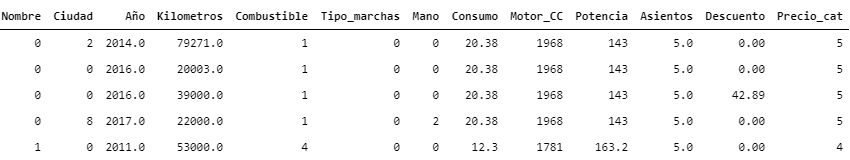
\includegraphics[scale=0.62]{img/data1.png}
\end{figure}

\begin{figure}[H]
    \centering
    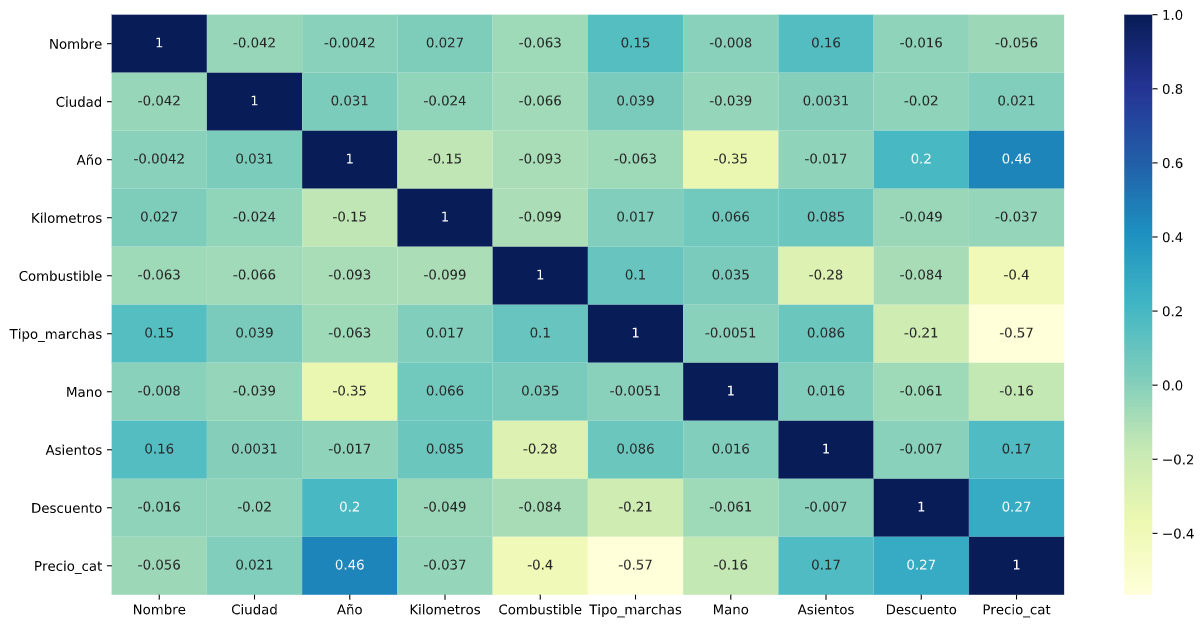
\includegraphics[scale=0.32]{img/corr.png}
\end{figure}

A continuación, pasamos a crear los modelos de clasificación. He introducido una pequeña sección de código que me sirve para
ejecutar unas pruebas rápidas de algún clasificador. Este código también lo utilizaré en los demás scripts.
\phantomsection
\label{rf}

\newpage
\begin{lstlisting}
    # Declaracion del modelo
    RndForestClf = RandomForestClassifier(n_estimators=100)
    
    # Calculo de las predicciones mediante validacion cruzada (5-folds)
    y_pred = cross_val_predict(RndForestClf, x_train, y_train, cv=5)
    
    print(classification_report(y_train, y_pred))
    print("SCORE: ", accuracy_score(y_train, y_pred))
    
    # Matriz de confusion de los resultados
    confusion_matrix = confusion_matrix(y_train, y_pred)
    
    sns.heatmap(confusion_matrix, annot = True, fmt='g')
\end{lstlisting}


En el código, lo que se hace es declarar y generar el modelo que vamos a testear, utilizar validación cruzada sobre el conjunto
de entrenamiento para ver cómo de eficaz es, y por último, mostramos las medidas de precisión obtenidas junto a su matriz de
confusión correspondiente.

Como ya he dicho, este código lo utilizaremos en scripts posteriores, sin embargo, en este primero no me fue tan útil, ya que
mi intención era probar cuantos más modelos mejor y me resultaba bastante tedioso hacerlo de esta forma. Para solucionarlo, cree
una lista de $pipelines$, en los cuales metía un modelo junto con los parámetros que quería probar. No tengo todos los modelos que
probé, pero si tengo las últimas pruebas con los que mejores resultados obtuve ($RandomForest$ y $MLPerceptron$). Este es el código
con el cual los generaba:

\phantomsection
\label{mlp}
\begin{lstlisting}
    # Crear lista de pipelines
    pipelines = []

    # Insertar nuevo pipeline
    for hidden_layer_sizes in hidden_layer_sizes_list :
        pipelines.append(
            make_pipeline(
                StandardScaler(),
                MLPClassifier(hidden_layer_sizes=hidden_layer_sizes,
                              early_stopping=False, random_state=1)
            )
        )
    nn_pipe = pipelines
\end{lstlisting}


Finalmente, para cada uno de los modelos de la lista, evaluamos su rendimiento he imprimimos tanto la media de aciertos como la
desviación típica que obtuvo cada uno. Además de esto, también se incluye una función que nos muestra una gráfica de la curva de
aprendizaje de cada uno de los modelos probados, y así poder analizar mejor cómo han funcionado nuestros algoritmos.

\begin{figure}[H]
    \centering
    
    \begin{minipage}{0.5\textwidth}
        \centering
        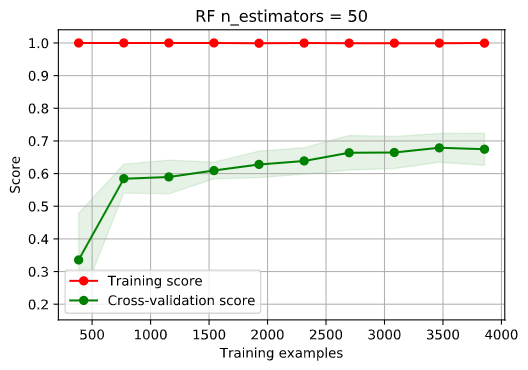
\includegraphics[scale=0.35]{img/lc1.png}
    \end{minipage}%
    \begin{minipage}{0.5\textwidth}
        \centering
        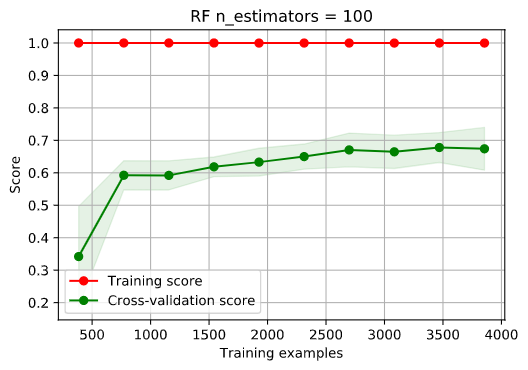
\includegraphics[scale=0.35]{img/lc2.png}
    \end{minipage}
    
\end{figure}
    
    
\begin{figure}[H]
    \centering
    
    \begin{minipage}{0.5\textwidth}
        \centering
        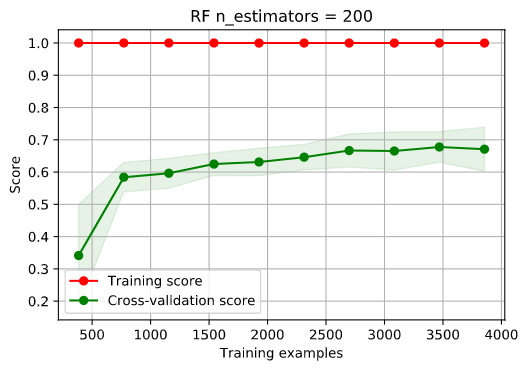
\includegraphics[scale=0.35]{img/lc3.png}
    \end{minipage}%
    \begin{minipage}{0.5\textwidth}
        \centering
        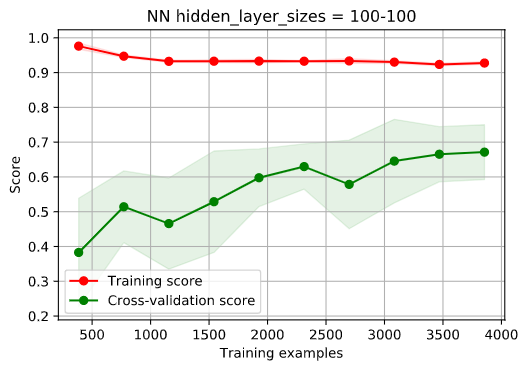
\includegraphics[scale=0.35]{img/lc4.png}
    \end{minipage}
    
\end{figure}

Podemos ver las curvas de aprendizaje de los modelos que mejores resultados obtuvieron. Como se puede apreciar, no son malas pero
como que el $score$ obtenido en la validación cruzada se estanca sobre el 70\%. No obstante, utilizamos el dataset de entrenamiento
hacer a su vez el test, asi que decidí probar a entrenar con todo entero y subir los resultados a la web.

Estos van a ser los ficheros 1 y 2 adjuntados en el zip (y en la tabla de soluciones), el primero con una red neuronal y el segundo
con el $random forest$.

Los resultados obtenidos no fueron los esperados, la verdad, ya que obtuve un 0.61518 para el $MLPerceptron$ y un 0.72131 para el
$RandomForest$. Por una parte, la puntuación de este último no me pareció muy mala, pese a que mi posición era de mitad de tabla
para abajo (no recuerdo muy bien estas primeras posiciones y tampoco las anoté). Pero por otra, me sorprendió la que obtuvo la red
neuronal, con un porcentaje mucho más bajo que el pronosticado y colocándome el penúltimo, si no recuerdo mal.


\subsection{Intentando mejorar los modelos}

Debido a los resultados obtenidos, intentamos mejorar el funcionamiento de los modelos, comenzando por el de la red neuronal. Mi
primera idea fue volver a probar más parámetros del $MLPerceptron$, pero como las pruebas rápidas realizadas continuaban dando
resultados similares, decidí cambiar de estrategia e implementar yo la red neuronal utilizando $Keras$:

\phantomsection
\label{rn}
\begin{lstlisting}
    # Build the model
    model = Sequential()

    model.add(Dense(10, input_shape=(12,), activation='relu'))
    model.add(Dense(10, activation='relu'))
    model.add(Dense(6, activation='sigmoid'))

    # Adam optimizer with learning rate of 0.0001
    optimizer = Adam(0.0001)
    model.compile(optimizer, loss='categorical_crossentropy',
                  metrics=['accuracy'])

\end{lstlisting}

Los parámetros para la red también fueron elegidos mediante pruebas rápidas y esos fueron los que mejor resultado dieron. Luego,
a la hora de subirlo a la web, la puntuación obtenida fue de 0.46764, lo cual ya me hizo pensar que la solución elegida no era
la correcta y que debía centrarme más en modelos como $RandomForest$, $AdaBoost$ o similares.

Ese mismo día probé a subir un $RandomForest$ con alguna pequeña modificación y con la cual obtuve un resultado de 0.69111.
Posteriormente, ya si probé a más opciones, y no sólo con parámetros de este clasificador, si no que también con los datos. 
La primera idea fue dejando la marca del coche (en vez de marca y modelo), cambiando el autocompletado de valores nulos
o no normalizando los datos finales. Sorprendentemente, lo que mejor resultado me dió fue esto último, aunque no entiendo muy bien
la razón. Igual fue por pérdida de información o porque no estaba normalizando bien; sin embargo, las tres subidas que hice ese día
obtuvieron una precisión del 0.71182, 0.75323 y 0.75150\footnote{De estas ejecuciones sólo conservo la que obtuvo mayor porcentaje,
las otras las he debido de eliminar sin querer}, colocándome en la posición 20 de 30 que estaban participando en ese momento,
aproximadamente.

\phantomsection
\label{prueba}
Las siguientes subidas un poco más de lo mismo. Intento cambiar parámetros y/o detalles del preprocesamiento a ver si mejoraba,
pero sin resultado alguno. Las primeras subidas del día 30 también pertenecen a estas pruebas y que, debido a las 3 subidas diarias,
no pude comprobar el día anterior. Más concretamente pertenecen al $StackingClassifier$, un método nuevo que consiste en 'apilar'
varios clasificadores en una salida perteneciente a un estimador final. Es decir, le pasamos varios clasificadores para calcular
la predicción final, y dependiendo de la fuerza que tenga cada clasificador individualmente, se utilizará su salida como entrada
de un estimador final (este será en mi caso $LogisticRegression()$, ya que es el más utilizado). Este clasificador junto con los
anteriormente explicados estarán en el notebook '\textit{mejorando-modelos.ipynb}':

\phantomsection
\label{stack}
\begin{lstlisting}
    # Clasificadores a apilar en el modelo
    estimators = [
        ('rf', RandomForestClassifier(n_estimators=100)),
        ('svr', make_pipeline(MinMaxScaler(),
                            LinearSVC()
                            )
        )]

    # Declaracion del modelo
    StackingClf = StackingClassifier(estimators=estimators,
                    final_estimator=LogisticRegression())
\end{lstlisting}

Si observamos los resultados en la web, no fueron muy buenos (0.70750 y 0.71786), algo que me resultó bastante extraño. Las pruebas
rápidas que hice con este modelo me dieron una precisión del 72\% más o menos. Teniendo en cuenta que se hace con validación
cruzada y que el conjunto con el que entrenamos se ve un poco más reducido, me resultó extraño. En este momento estaba un poco
bloqueado, por lo que decidí cambiar el planteamiento totalmente y empezar de nuevo.


\subsection{Cambiando el planteamiento}

Viendo que mis resultados no mejoraban y que también estaba bajando bastantes posiciones en la tabla (iría ya por la posición 30-35
de ya unas 40 personas que hay), me hicieron pensar que no todo era el clasificador que estaba utilizando, sino que el preprocesado
de los datos también influye bastante en el resultado final.

Me estuve leyendo las transparencias, viendo las prácticas anteriores y buscando un por internet para informarme en qué podía
mejorar (sobre todo me ayudó una pequeña conferencia conferencia de la Universidad de DePaul \cite{bib:depaul-uni}). El comienzo es
muy similar al anterior, quitando la columna de las etiquetas y las unidades de los datos como los 'kmpl' o 'bhp'. La única
diferencia es que meto los datos de entrenamiento y test en el mismo $DataFrame$, para así no tener que repetir el preprocesado.

\phantomsection
\label{pp3}
Los cambios que vienen a continuación estarán en el notebook '\textit{guion-final.ipynb}'. Lo primero que hacemos es ver la
cantidad de variables categóricas que tenemos y decidir cuales vamos a utilizar. En principio, sólo el nombre o marca del vehículo
es la que más categorías únicas tiene, por lo que es la que nos planteamos si quitar o mantener (a priori la quitaremos). Lo
siguiente que vemos es que la categoría 'Combustible' predominan las de tipo $Diesel$ y $Petrol$, por lo que el resto que no sean
de ese tipo, las clasificaremos como $Other$.

A continuación, vamos a transformar estas variables categóricas en variables '$dummy$', es decir, variables numéricas mediante una
serie de ceros y unos.

\begin{figure}[H]
    \centering
    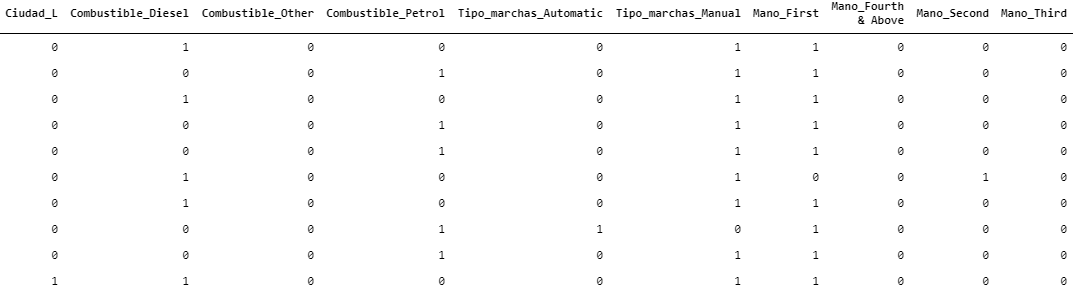
\includegraphics[scale=0.5]{img/dummy.png}
\end{figure}

Ahora pasamos a tratar los datos incorrectos o que faltan. Esta vez, lo vamos a hacer de una forma distinta a la anterior. Vamos a
rellenar los datos que faltan en una columna, utilizando la mediana de esos datos en esa misma columna. Con el descuento, al igual
que hicimos anteriormente, pienso que es mejor completarlos con un 0.

Algo nuevo que haremos será tratar los valores con ruido o $outliers$. Para ello vamos a utilizar la siguiente función:

\begin{lstlisting}
    def find_outliers(x):
        q1 = np.percentile(x, 25)
        q3 = np.percentile(x, 75)
        iqr = q3-q1
        floor = q1 - 1.75*iqr
        ceiling = q3 + 1.75*iqr
        outlier_indices = list(x.index[(x < floor)|(x > ceiling)])
        outlier_values = list(x[outlier_indices])

    return outlier_indices, outlier_values
\end{lstlisting}

En ella obtenemos un valor para los cuartiles 1 y 3 (podemos ajustarlo manualmente para hacerlo más o menos restrictivo), e
imprimimos los valores que queden fuera de este rango. Gracias a esto, podemos observar que, en los kilómetros por ejemplo, hay
un coche con 6 millones de kilómetros realizados, lo cual es prácticamente imposible. Se ha seleccionado un valor umbral de medio
millón de kilómetros realizados para que selecciones estos valores como ruido (con más de 300.000 suelen ir a desguace en vez de
venderse). También se han ajustado otros valores como el consumo, en el algunos coches tenían un 0.

Lo siguiente que se ha realizado ha sido añadir interacciones entre características. Esto puede resultar muy útil, ya que añadimos
más características a nuestro modelo que pueden potenciar el resultado si los atributos generan alguna relación. Hay que tener en
cuenta que las interacciones entre variables que pertenecen a la misma variable categórica, son siempre cero. Para llevarlo a
cabo, se ha utilizado '$PolynomialFeatures$', una función de $sklearn$ cuyo funcionamiento será más fácil de comprender si se mira
en la página oficial \cite{bib:polynomialfeatures}.

Tras realizar todo este preprocesado, hemos obtenido una cantidad de 970 columnas en nuestro dataset. Esto nos lleva a la siguiente
parte del código, que es la reducción de dimensionalidad mediante PCA o selección de características ($SelectKBest$). Esto
finalmente no se va a utilizar, ya que estaba pensado para hacer algún intento más utilizando redes neuronales, y no ha sido
posible.

Las pruebas que se han realizado con estos datos son bastante más de las que se han llegado a subir (las añadire todas al zip), ya
que las subidas diarias limitaban el poder probar cada cambio. Pese a esto, no creo que fuesen mucho mejores de las que ya hay,
ya que en la prueba rápida realizada, los valores se mantenían más o menos similares.

Para empezar se probó el último modelo visto, $StackingClassifier$, con la misma configuración, para así tener una referencia de
si estaba funcionando o no. El resultado fue bastante bueno, ya que obtuve un 0.77825, colocándome el 18 en la clasificación.
Esto quería decir que los cambios en los datos habían funcionado.

\phantomsection
\label{grid}
En la tabla del siguiente punto explicaré los detalles entre unas subidas y otra, pero los cambios o pruebas más relevante que
hice, me gustaría comentarlas ahora. Uno de ellos fue la búsqueda automática de hiperparámetros para nuestro modelo. Esto lo he
hecho gracias a $GridSearchCV$, una función al la que le introducimos una serie de hiperparámetros para un modelo y, mediante
validación cruzada, selecciona los que mejores resultados han ofrecido:

\begin{lstlisting}
    # Creacion del grid de parametros
    param_grid = {
        'criterion': ['gini'],
        'max_depth': [None],
        'min_samples_leaf': [1, 2, 3, 4, 5],
        'min_samples_split': [2, 3, 4, 5, 6],
        'n_estimators': [100, 150, 175, 200]
    }

    # Entrenamos el modelo con las distintas opciones
    gs = GridSearchCV(estimator=rf, param_grid=param_grid,
                      cv=5, n_jobs=-1, verbose=1)
    gs = gs.fit(x_train, y_train)

    # Imprimimos los mejores resultados
    print(gs.best_score_)
    print(gs.best_params_)

    # Creamos el modelos con los parametros elegidos
    bp = gs.best_params_
    RndForestClf = RandomForestClassifier(criterion=bp['criterion'],
                            min_samples_leaf=bp['min_samples_leaf'],
                            min_samples_split=bp['min_samples_split'],
                            max_depth=bp['max_depth'],
                            n_estimators=bp['n_estimators'])
\end{lstlisting}

Este ejemplo calcula unos parametros para el $RandomForest$, con el cual realizaría tres subidas (aunque tienen algunos cambios
en el preprocesado que explicare en la tabla) que me dieron un resultado de 0.76617, 0.76186 y 0.76531. Valores muy similares al
anterior pero con los que no conseguí mejorar.

La siguiente subida sería con la que he alcazado mi posición final. Lo que he hecho ha sido utilizar el $GridSearchCV$ para
generar un modelo de \textit{\textbf{RandomForest}}, y a su vez, meterlo dentro de un \textit{\textbf{StackingClassifier}} junto
con un una \textit{\textbf{Linear Support Vector Machine}}. La idea la he sacado del propio manual del $StackingClassifier$
\cite{bib:stacking}. Sinceramente, todavía me esperaba un mejor resultado, ya que en las pruebas rápida realizada he alcanzado
un valor de hasta 82-85\% de precisión, y según la tendencia de estos experimentos rápidos, este valor solía ser menor que el
obtenido finalmente en la web. Aun así, el $accuracy$ obtenido ha sido de 0.79119, con el que conseguí la posición 12 si no
recuerdo mal.

Otro cambio bastante sustancial para las últimas ejecuciones fue el de introducir aún más modelos en el $StackingClassifier$:

\begin{lstlisting}
    estimators = [
        ('lr', LogisticRegression()),
        ('RndForestClf', RndForestClf),
        ('svr', make_pipeline(StandardScaler(), LinearSVC()) ),
        ('bayes', GaussianNB())
    ]

    StackingClf = StackingClassifier(estimators=estimators, final_estimator=LogisticRegression())
\end{lstlisting}

y también una última versión con un ExtraTreeClassifier con una búsqueda de parámetros antes, pero no mejoró el resultado.

Finalmente, comentar que me habría gustado probar bastantes más opciones y modelos, como pueden ser las redes neuronales con este
último preprocesado, probar con la reducción de características o investigar si encuentro alguna forma de conseguir mejorar el
que ya tengo. No obstante, estoy bastante contento con el resultado final, ya que no he tenido mucho tiempo y siento que el
resultado ha sido bastante competitivo (está a un 4\% de precisión aproximadamente del mejor).

\section{Tabla de soluciones}

Las palabras subrayadas te llevarán a la explicación completa en la memoria. Los valores con un '-' es porque al no mejorar, la
posición sería la misma o más baja, ya que si mejoraba algún otro alumno, cambiaría. (posición/total de alumnos).

% Please add the following required packages to your document preamble:
% \usepackage{graphicx}
\begin{table}[H]
    \centering
    \resizebox{\textwidth}{!}{%
    \begin{tabular}{|c|c|c|c|c|c|}
    \hline
    \textbf{Fecha} & \textbf{Posición} & \textbf{Train/Test score} & \textbf{Descripción preprocesado} & \textbf{Descripción método} & \textbf{Parámetros} \\ \hline
    Dec 26 - 03:34 & 20/22 & \begin{tabular}[c]{@{}c@{}}0.685602\\ 0.61518\end{tabular} & \begin{tabular}[c]{@{}c@{}}Preprocesado de prueba\\ explicado en la sección \ref{pp1}\end{tabular} & \begin{tabular}[c]{@{}c@{}}Red neuronal en forma\\ de \hyperref[mlp]{\underline{MLPerceptron}}\end{tabular} & hidden\_layer\_sizes = (100,100) \\ \hline
    Dec 26 - 04:00 & 16/22 & \begin{tabular}[c]{@{}c@{}}0.671908\\ 0.72131\end{tabular} & \begin{tabular}[c]{@{}c@{}}Preprocesado de prueba\\ explicado en la sección \ref{pp1}\end{tabular} & \hyperref[rf]{\underline{Random Forest}} por defecto & n\_estimators = 200 \\ \hline
    Dec 27 - 02:56 & - & \begin{tabular}[c]{@{}c@{}}0.7462\\ 0.46764\end{tabular} & \begin{tabular}[c]{@{}c@{}}Preprocesado de prueba\\ explicado en la sección \ref{pp1}\end{tabular} & \hyperref[rn]{\underline{Red neuronal}} hecha a mano & \begin{tabular}[c]{@{}c@{}}Capas dense de (12-10-10-6)\\ optimizer = Adam(0.0001)\\ activation = 'sigmoid'\end{tabular} \\ \hline
    Dec 27 - 03:04 & - & \begin{tabular}[c]{@{}c@{}}0.69864\\ 0.69111\end{tabular} & \begin{tabular}[c]{@{}c@{}}Preprocesado de prueba\\ explicado en la sección \ref{pp1}\end{tabular} & \hyperref[rf]{\underline{Random Forest}} por defecto & \begin{tabular}[c]{@{}c@{}}n\_estimators = 100\\ max\_depth = None\end{tabular} \\ \hline
    Dec 28 - 22:30 & - & \begin{tabular}[c]{@{}c@{}}0.71232\\ 0.71182\end{tabular} & \begin{tabular}[c]{@{}c@{}}Preprocesado de prueba\\ con pequeñas \hyperref[prueba]{\underline{modificaciones}}\end{tabular} & \hyperref[rf]{\underline{Random Forest}} por defecto & \begin{tabular}[c]{@{}c@{}}n\_estimators = 100\\ max\_depth = None\\ (obtuvieron mejor resultado\\ en el train que el anterior)\end{tabular} \\ \hline
    Dec 28 - 22:34 & 20/30 & \begin{tabular}[c]{@{}c@{}}0.71156\\ 0.75323\end{tabular} & \begin{tabular}[c]{@{}c@{}}Preprocesado de prueba\\ con pequeñas \hyperref[prueba]{\underline{modificaciones}}\end{tabular} & \hyperref[rf]{\underline{Random Forest}} por defecto & \begin{tabular}[c]{@{}c@{}}n\_estimators = 100\\ max\_depth = None\\ (obtuvieron mejor resultado\\ en el train que el anterior)\end{tabular} \\ \hline
    Dec 28 - 22:39 & - & \begin{tabular}[c]{@{}c@{}}0.72455\\ 0.75150\end{tabular} & \begin{tabular}[c]{@{}c@{}}Preprocesado de prueba\\ con pequeñas \hyperref[prueba]{\underline{modificaciones}}\end{tabular} & \hyperref[rf]{\underline{Random Forest}} por defecto & \begin{tabular}[c]{@{}c@{}}n\_estimators = 100\\ max\_depth = None\\ (obtuvieron mejor resultado\\ en el train que el anterior)\end{tabular} \\ \hline
    Dec 29 - 01:17 & - & \begin{tabular}[c]{@{}c@{}}0.72463\\ 0.74719\end{tabular} & \begin{tabular}[c]{@{}c@{}}Preprocesado de prueba\\ con pequeñas \hyperref[prueba]{\underline{modificaciones}}\end{tabular} & \begin{tabular}[c]{@{}c@{}}\hyperref[stack]{\underline{Stacking Classifier}} con un\\ Random Forest y LinearSVC\end{tabular} & \begin{tabular}[c]{@{}c@{}}final\_estimator =\\ LogisticRegression()\end{tabular} \\ \hline
    Dec 29 - 01:33 & - & \begin{tabular}[c]{@{}c@{}}0.72003\\ 0.75237\end{tabular} & \begin{tabular}[c]{@{}c@{}}Preprocesado de prueba\\ con pequeñas \hyperref[prueba]{\underline{modificaciones}}\end{tabular} & \begin{tabular}[c]{@{}c@{}}\hyperref[stack]{\underline{Stacking Classifier}} con un\\ Random Forest y LinearSVC\end{tabular} & \begin{tabular}[c]{@{}c@{}}final\_estimator =\\ LogisticRegression(max\_iter =\\ 10000, tol = 1e-5)\end{tabular} \\ \hline
    Dec 29 - 02:47 & - & \begin{tabular}[c]{@{}c@{}}0.69329\\ 0.63589\end{tabular} & \begin{tabular}[c]{@{}c@{}}Preprocesado de prueba\\ con pequeñas \hyperref[prueba]{\underline{modificaciones}}\end{tabular} & \begin{tabular}[c]{@{}c@{}}\hyperref[stack]{\underline{Stacking Classifier}} con un\\ AdaBoostClasifier, SVC y\\ SGDClassifier\end{tabular} & \begin{tabular}[c]{@{}c@{}}final\_estimator =\\ LogisticRegression()\end{tabular} \\ \hline
    Dec 30 - 01:00 & - & \begin{tabular}[c]{@{}c@{}}0.72387\\ 0.70750\end{tabular} & \begin{tabular}[c]{@{}c@{}}Preprocesado de prueba\\ con pequeñas \hyperref[prueba]{\underline{modificaciones}}\\ Añadimos nombre y marca\\ del coche\end{tabular} & \begin{tabular}[c]{@{}c@{}}\hyperref[stack]{\underline{Stacking Classifier}} con un\\ Random Forest y LinearSVC\end{tabular} & \begin{tabular}[c]{@{}c@{}}final\_estimator =\\ LogisticRegression()\end{tabular} \\ \hline
    Dec 30 - 01:33 & - & \begin{tabular}[c]{@{}c@{}}0.72546\\ 0.71786\end{tabular} & \begin{tabular}[c]{@{}c@{}}Preprocesado de prueba\\ con pequeñas \hyperref[prueba]{\underline{modificaciones}}\\ Utilizamos MinMaxScaler para\\ normalizar los datos\end{tabular} & \begin{tabular}[c]{@{}c@{}}\hyperref[stack]{\underline{Stacking Classifier}} con un\\ Random Forest y LinearSVC\end{tabular} & \begin{tabular}[c]{@{}c@{}}final\_estimator =\\ LogisticRegression()\end{tabular} \\ \hline
    Dec 30 - 19:15 & 18/40 & \begin{tabular}[c]{@{}c@{}}0.81402\\ 0.77825\end{tabular} & \begin{tabular}[c]{@{}c@{}}Nuevo preprocesado más\\ complejo y con bastantes\\ detalle resumidos \hyperref[pp3]{\underline{aqui}}\end{tabular} & \begin{tabular}[c]{@{}c@{}}\hyperref[stack]{\underline{Stacking Classifier}} con un\\ Random Forest y LinearSVC\end{tabular} & \begin{tabular}[c]{@{}c@{}}final\_estimator =\\ LogisticRegression()\end{tabular} \\ \hline
    Dec 31 - 01:02 & - & \begin{tabular}[c]{@{}c@{}}0.80722\\ 0.76617\end{tabular} & \begin{tabular}[c]{@{}c@{}}Nuevo preprocesado más\\ complejo y con bastantes\\ detalle resumidos \hyperref[pp3]{\underline{aqui}}\\ Se procesan los datos\\ con ruido\end{tabular} & \hyperref[rf]{\underline{Random Forest}} por defecto & \begin{tabular}[c]{@{}c@{}}Búsqueda de parámetros\\ con \hyperref[grid]{\underline{GridSearchCV}}\end{tabular} \\ \hline
    Dec 31 - 01:03 & - & \begin{tabular}[c]{@{}c@{}}0.81531\\ 0.76186\end{tabular} & \begin{tabular}[c]{@{}c@{}}Nuevo preprocesado más\\ complejo y con bastantes\\ detalle resumidos \hyperref[pp3]{\underline{aqui}}\\ Se procesan los datos\\ con ruido\end{tabular} & \hyperref[rf]{\underline{Random Forest}} por defecto & \begin{tabular}[c]{@{}c@{}}Búsqueda de parámetros\\ con \hyperref[grid]{\underline{GridSearchCV}}\\ El criterion='entropy', que\\ fue lo más destacable\end{tabular} \\ \hline
    Dec 31 - 01:24 & - & \begin{tabular}[c]{@{}c@{}}0.81531\\ 0.76531\end{tabular} & \begin{tabular}[c]{@{}c@{}}Nuevo preprocesado más\\ complejo y con bastantes\\ detalle resumidos \hyperref[pp3]{\underline{aqui}}\\ Se procesa el ruido\\ Añadimos la columna nombre\end{tabular} & \hyperref[rf]{\underline{Random Forest}} por defecto & \begin{tabular}[c]{@{}c@{}}Búsqueda de parámetros\\ con \hyperref[grid]{\underline{GridSearchCV}}\end{tabular} \\ \hline
    \textbf{Jan 1 - 18:09} & \textbf{12/45} & \textbf{\begin{tabular}[c]{@{}c@{}}0.82998\\ 0.79119\end{tabular}} & \textbf{\begin{tabular}[c]{@{}c@{}}Nuevo preprocesado más\\ complejo y con bastantes\\ detalle resumidos \hyperref[pp3]{\underline{aqui}}\\ Se procesa el ruido\\ Añadimos la columna nombre\end{tabular}} & \textbf{\begin{tabular}[c]{@{}c@{}}\hyperref[stack]{\underline{Stacking Classifier}} con un\\ Random Forest y LinearSVC\end{tabular}} & \textbf{\begin{tabular}[c]{@{}c@{}}Búsqueda de parámetros del\\ RandomForest utilizado\\ con \hyperref[grid]{\underline{GridSearchCV}}\end{tabular}} \\ \hline
    Jan 1 - 22:06 & - & \begin{tabular}[c]{@{}c@{}}0.82444\\ 0.78602\end{tabular} & \begin{tabular}[c]{@{}c@{}}Nuevo preprocesado más\\ complejo y con bastantes\\ detalle resumidos \hyperref[pp3]{\underline{aqui}}\\ Se procesa el ruido\\ Añadimos la columna nombre\end{tabular} & \begin{tabular}[c]{@{}c@{}}\hyperref[stack]{\underline{Stacking Classifier}} con un\\ LogisticRegression, Random Forest,\\ LinearSVC y GaussianNB\end{tabular} & \begin{tabular}[c]{@{}c@{}}Búsqueda de parámetros del\\ RandomForest utilizado\\ con \hyperref[grid]{\underline{GridSearchCV}}\end{tabular} \\ \hline
    Jan 1 - 22:37 & - & \begin{tabular}[c]{@{}c@{}}0.82238\\ 0.78774\end{tabular} & \begin{tabular}[c]{@{}c@{}}Nuevo preprocesado más\\ complejo y con bastantes\\ detalle resumidos \hyperref[pp3]{\underline{aqui}}\\ Se procesa el ruido\\ Añadimos la columna nombre\end{tabular} & \begin{tabular}[c]{@{}c@{}}\hyperref[stack]{\underline{Stacking Classifier}} con un\\ LogisticRegression, Random Forest,\\ ExtraTreeClassifier,\\ LinearSVC y GaussianNB\end{tabular} & \begin{tabular}[c]{@{}c@{}}Búsqueda de parámetros del\\ RandomForest utilizado\\ con \hyperref[grid]{\underline{GridSearchCV}}\end{tabular} \\ \hline
    \end{tabular}%
    }
    \end{table}

\newpage

% Pagina de bibliografia
\begin{thebibliography}{}

    
    \bibitem{bib:svc}
    Scikit-Learn \textit{SVC}
    \\\url{https://scikit-learn.org/stable/modules/generated/sklearn.svm.SVC.html#sklearn.svm.SVC}
    
    \bibitem{bib:random_forest}
    Scikit-Learn \textit{RandomForestClassifier}
    \\\url{https://scikit-learn.org/stable/modules/generated/sklearn.ensemble.RandomForestClassifier.html#sklearn.ensemble.RandomForestClassifier}
    
    \bibitem{bib:stacking}
    Scikit-Learn \textit{StackingClassifier}
    \\\url{https://scikit-learn.org/stable/modules/generated/sklearn.ensemble.StackingClassifier.html}
    
    \bibitem{bib:neural_network}
    Scikit-Learn \textit{MLPClassifier}
    \\\url{https://scikit-learn.org/stable/modules/generated/sklearn.neural_network.MLPClassifier.html#sklearn.neural_network.MLPClassifier}
    
    \bibitem{bib:learning_curve}
    Scikit-Learn \textit{plot\_learning\_curve}
    \\\url{https://scikit-learn.org/stable/auto_examples/model_selection/plot_learning_curve.html#sphx-glr-auto-examples-model-selection-plot-learning-curve-py}
    
    \bibitem{bib:loss-nn}
    Isaac Changhau. \textit{Loss Functions in Neural Networks}
    \\\url{https://isaacchanghau.github.io/post/loss_functions/}

    \bibitem{bib:depaul-uni}
    DePaul University.
    \\\url{http://mdp.cdm.depaul.edu/DePy2016}

    \bibitem{bib:scaler}
    Scikit-Learn. \textit{StandardScaler}
    \\\url{https://scikit-learn.org/stable/modules/generated/sklearn.preprocessing.StandardScaler.html}
    
    \bibitem{bib:pca}
    Scikit-Learn \textit{PCA}
    \\\url{https://scikit-learn.org/stable/modules/generated/sklearn.decomposition.PCA.html}
    
    \bibitem{bib:polynomialfeatures}
    Scikit-Learn \textit{PolynomialFeatures}
    \\\url{https://scikit-learn.org/stable/modules/generated/sklearn.preprocessing.PolynomialFeatures.html}

    \bibitem{bib:svm}
    Scikit-Learn \textit{GridSearchCV}
    \\\url{https://scikit-learn.org/stable/modules/generated/sklearn.model_selection.GridSearchCV.html}
    
    \bibitem{bib:svm}
    MathWorks \textit{Support Vector Machine}
    \\\url{https://es.mathworks.com/discovery/support-vector-machine.html}
    
    \bibitem{bib:cross_val_score}
    Scikit-Learn \textit{cross\_val\_score}
    \\\url{https://scikit-learn.org/stable/modules/generated/sklearn.model_selection.cross_val_score.html}
    
    \bibitem{bib:train_test_split}
    Scikit-Learn \textit{train\_test\_split}
    \\\url{https://scikit-learn.org/stable/modules/generated/sklearn.model_selection.train_test_split.html}
    
    \bibitem{bib:confusion-matrix}
    Scikit-Learn \textit{Confusion Matrix}
    \\\url{https://scikit-learn.org/stable/auto_examples/model_selection/plot_confusion_matrix.html}
    
    \end{thebibliography}



\end{document}